\documentclass[a4paper,5pt]{amsbook}
%%%%%%%%%%%%%%%%%%%%%%%%%%%%%%%%%%%%%%%%%%%%%%%%%%%%%%%%%%%%%%%%%%%%%

%\usepackage{booktabs}
\usepackage{graphicx}
%\usepackage{multicol}
%\usepackage{textcomp}
%\usepackage{systeme}
%\usepackage{amssymb}
%\usepackage[]{amsmath}
%\usepackage{subcaption}
\usepackage[inline]{enumitem}
%\usepackage{gensymb}

%%%%%%%%%%%%%%%%%%%%%%%%%%%%%%%%%%%%%%%%%%%%%%%%%%%%%%%%%%%%%%

\newcommand{\sen}{\,\mbox{sen}\,}
\newcommand{\tg}{\,\mbox{tg}\,}
\newcommand{\cosec}{\,\mbox{cosec}\,}
\newcommand{\cotg}{\,\mbox{cotg}\,}
\newcommand{\tr}{\,\mbox{tr}\,}
\newcommand{\ds}{\displaystyle}
\newcommand{\ra}{\rightarrow}

%%%%%%%%%%%%%%%%%%%%%%%%%%%%%%%%%%%%%%%%%%%%%%%%%%%%%%%%%%%%%%%%%%%%%%%%

\setlength{\textwidth}{16cm} \setlength{\topmargin}{-1.7cm}
\setlength{\textheight}{25cm}
\setlength{\leftmargin}{1.2cm} \setlength{\rightmargin}{1.2cm}
\setlength{\oddsidemargin}{0cm}\setlength{\evensidemargin}{0cm}

%%%%%%%%%%%%%%%%%%%%%%%%%%%%%%%%%%%%%%%%%%%%%%%%%%%%%%%%%%%%%%%%%%%%%%%%

% \renewcommand{\baselinestretch}{1.6}
% \renewcommand{\thefootnote}{\fnsymbol{footnote}}
% \renewcommand{\theequation}{\thesection.\arabic{equation}}
% \setlength{\voffset}{-50pt}
% \numberwithin{equation}{chapter}

%%%%%%%%%%%%%%%%%%%%%%%%%%%%%%%%%%%%%%%%%%%%%%%%%%%%%%%%%%%%%%%%%%%%%%%

\begin{document}
\thispagestyle{empty}
\pagestyle{empty}
\begin{minipage}[h]{0.14\textwidth}
	
\includegraphics[scale=0.24]{../ufgd.png}
\end{minipage}
\begin{minipage}[h]{\textwidth}
\begin{tabular}{c}
{{\bf UNIVERSIDADE FEDERAL DA GRANDE DOURADOS}}\\
{{\bf C\'alculo Diferencial e Integral --- Lista 14}}\\
{{\bf Prof.\ Adriano Barbosa}}\\
\end{tabular}
\vspace{-0.45cm}
%
\end{minipage}

%------------------------

\vspace{1cm}
%%%%%%%%%%%%%%%%%%%%%%%%%%%%%%%%   formulario  inicio  %%%%%%%%%%%%%%%%%%%%%%%%%%%%%%%%
\begin{enumerate}
    \item O gr\'afico de $g$ consiste em duas retas e um semic\'{i}rculo. Use-o
        para calcular cada integral

    \begin{enumerate*}
    	\item $\displaystyle\int_0^2 g(x)\ dx$
        \hspace{0.3cm}
        \hspace{0.3cm}
    	\item $\displaystyle\int_2^6 g(x)\ dx$
        \hspace{0.3cm}
        \hspace{0.3cm}
    	\item $\displaystyle\int_0^6 g(x)\ dx$
    \end{enumerate*}
    
    \begin{figure}[h]
    	\centering
    	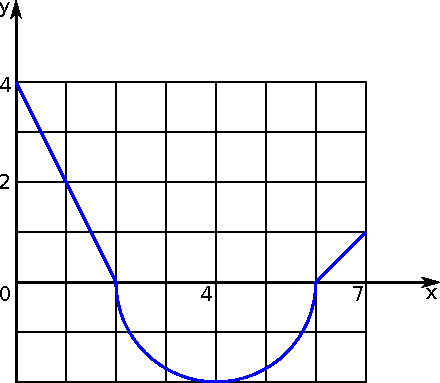
\includegraphics[scale=0.7]{lista-14-fig1.pdf}
    \end{figure}
    
    \vspace{0.5cm}
    \item Calcule as integrais interpretando-as em termos de \'areas.

    \begin{enumerate*}
    	\item $\displaystyle\int_{-1}^2 1 - x\ dx$
        \hspace{0.3cm}
        \hspace{0.3cm}
    	\item $\displaystyle\int_{-1}^2 |x|\ dx$
    \end{enumerate*}
    
    \vspace{0.5cm}
    \item Apenas analisando o gr\'afico das fun\c{c}\~oes, calcule as seguintes integrais

    \begin{enumerate*}
    	\item $\displaystyle\int_{-1}^1 x\ dx$
        \hspace{0.1cm}
        \hspace{0.1cm}
    	\item $\displaystyle\int_{-1}^1 |t|\ dt$
        \hspace{0.1cm}
        \hspace{0.1cm}
    	\item $\displaystyle\int_{-1}^1 y^2\ dy$
        \hspace{0.1cm}
        \hspace{0.1cm}
    	\item $\displaystyle\int_{-\pi}^{\pi} \sin\theta\ d\theta$
        \hspace{0.1cm}
        \hspace{0.1cm}
    	\item $\displaystyle\int_{-\pi}^{\pi} \cos\phi\ d\phi$
    \end{enumerate*}

    \vspace{0.5cm}
    \item Use o Teorema Fundamental do C\'alculo para encontrar a derivada das
    	fun\c{c}\~oes abaixo
    \begin{enumerate}
    	\item $\displaystyle g(x) = \int_1^x \frac{1}{t^3 + 1}\ dt$
    	\item $\displaystyle G(x) = \int_x^1 \cos(\sqrt{t})\ dt$
        \item $\displaystyle h(x) = \int_{2x}^{3x} \frac{u^2 - 1}{u^2 + 1}\ du$
            (dica: use as propriedades de integrais e a regra da cadeia.)
    \end{enumerate}
\end{enumerate}

\end{document}
